\documentclass[aspectratio=169]{beamer}
\setbeamertemplate{navigation symbols}{}
\usepackage{color, amsmath, comment, subfigure}
\usepackage{url}
\usepackage{ulem}

\usepackage{hyperref}
\hypersetup{
    colorlinks=true,
    linkcolor=blue,
    filecolor=magenta,      
    urlcolor=cyan,
}

%%%%%%%%%%%%%%%%%%%%%%%%%%
\title[]{Class slides for Thursday, October 24:\\Weather, Empirical}
\author[]{Matthew J. Salganik}
\institute[]{}
\date[]{COS 597E/SOC 555 Limits to prediction\\Fall 2020, Princeton University}

\begin{document}
%%%%%%%%%%%%%%%%%%%%%%%%%%%
\frame{\titlepage}
%%%%%%%%%%%%%%%%%%%%%%%%%%%
\begin{frame}
\frametitle{}

\begin{align*}
  x' &= \sigma(y-x) \\
  y' &= x(\rho-z)-y \\
  z' &= xy-\beta z
\end{align*}
\begin{center}
$\sigma = 10, \rho = 28,  \beta = 8/3$ 
\end{center}
\begin{center}
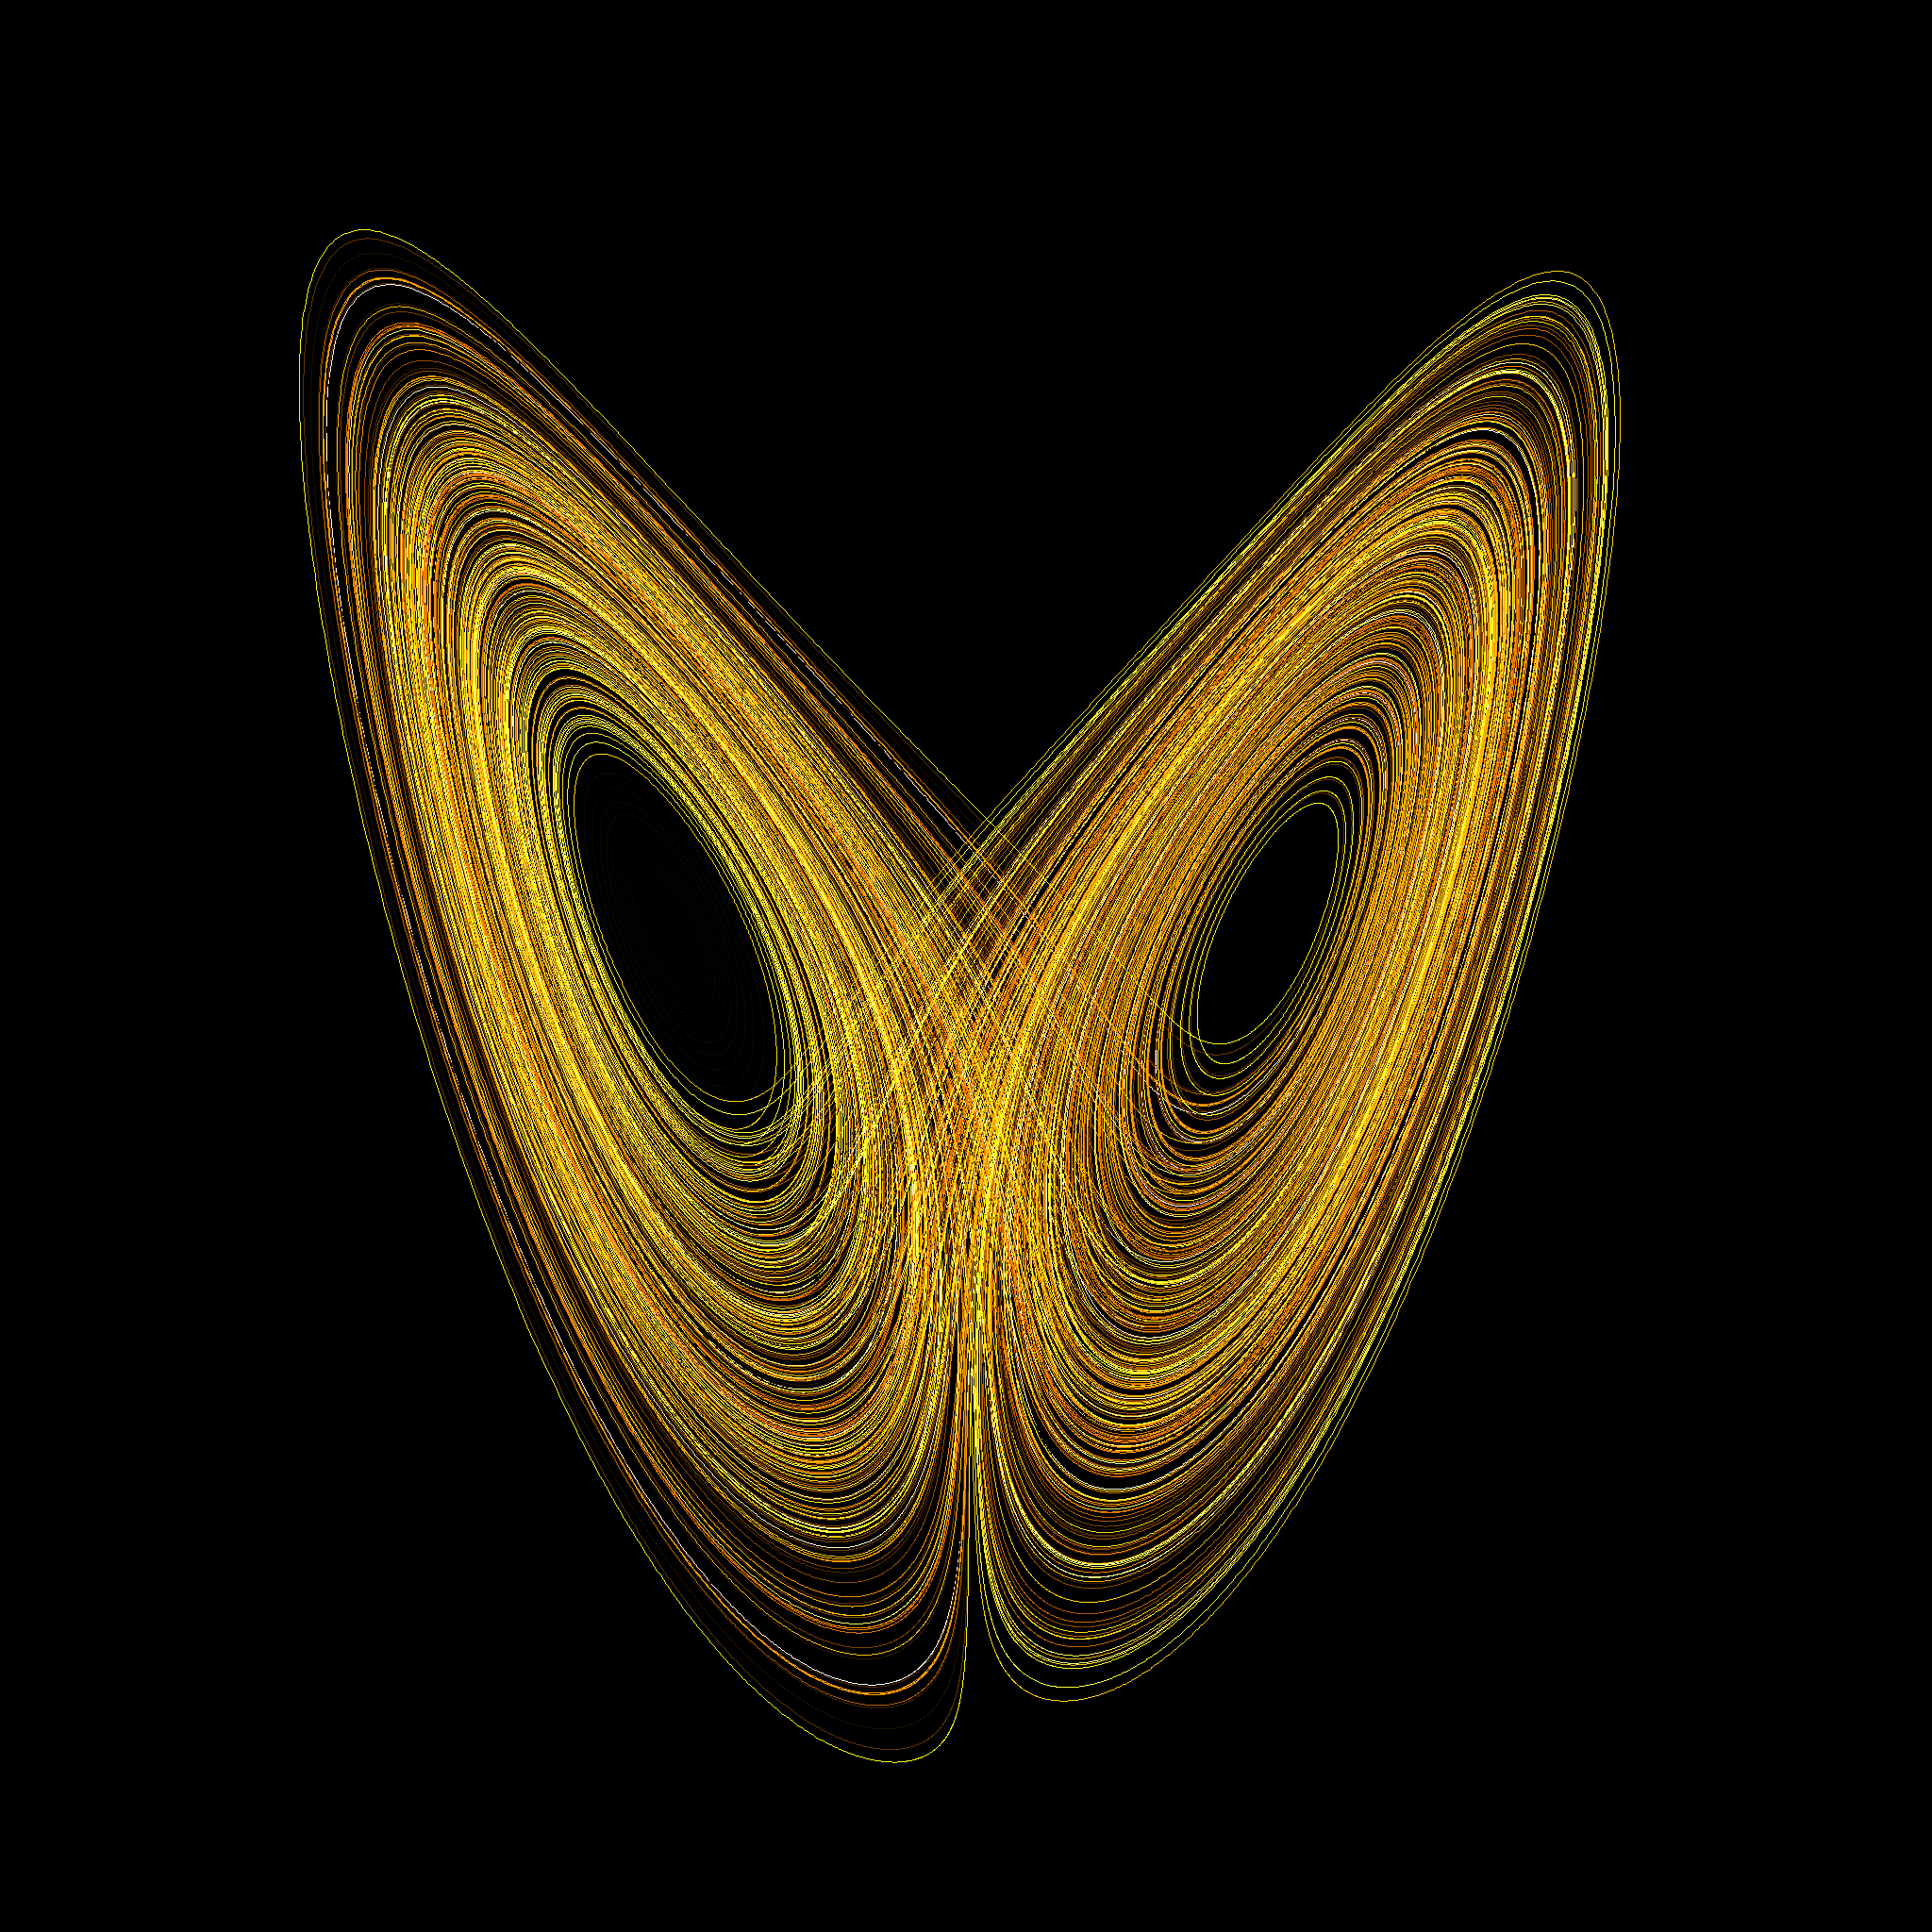
\includegraphics[width = 0.3\textwidth]{figures/Lorenz_system_r28_s10_b2-6666}
\end{center}

\vfill
\tiny{\url{https://commons.wikimedia.org/wiki/File:Lorenz_system_r28_s10_b2-6666.png}}
\end{frame}
%%%%%%%%%%%%%%%%%%%%%%%%%%%%%
\begin{frame}
\frametitle{}

\begin{center}
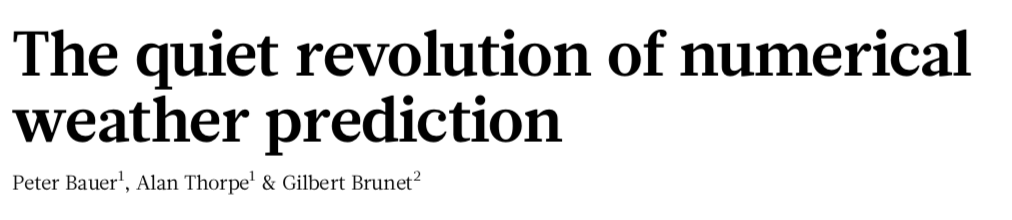
\includegraphics[width = 0.9\textwidth]{figures/bauer_quiet_2015_title}
\end{center}

\end{frame}
%%%%%%%%%%%%%%%%%%%%%%%%%%%%%
\begin{frame}

\begin{center}
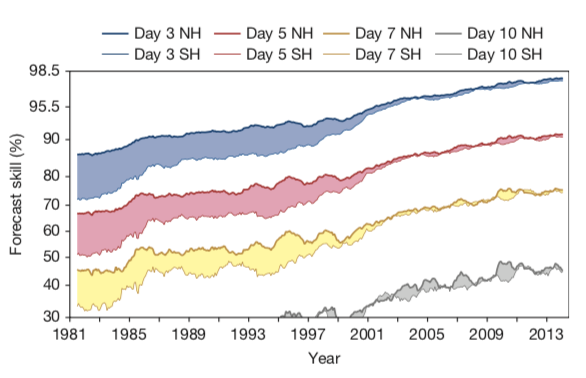
\includegraphics[width = 0.8\textwidth]{figures/bauer_quiet_2015_fig1}
\end{center}

\vfill
This is impressive.

\end{frame}
%%%%%%%%%%%%%%%%%%%%%%%%%%%%%
\begin{frame}

\begin{center}
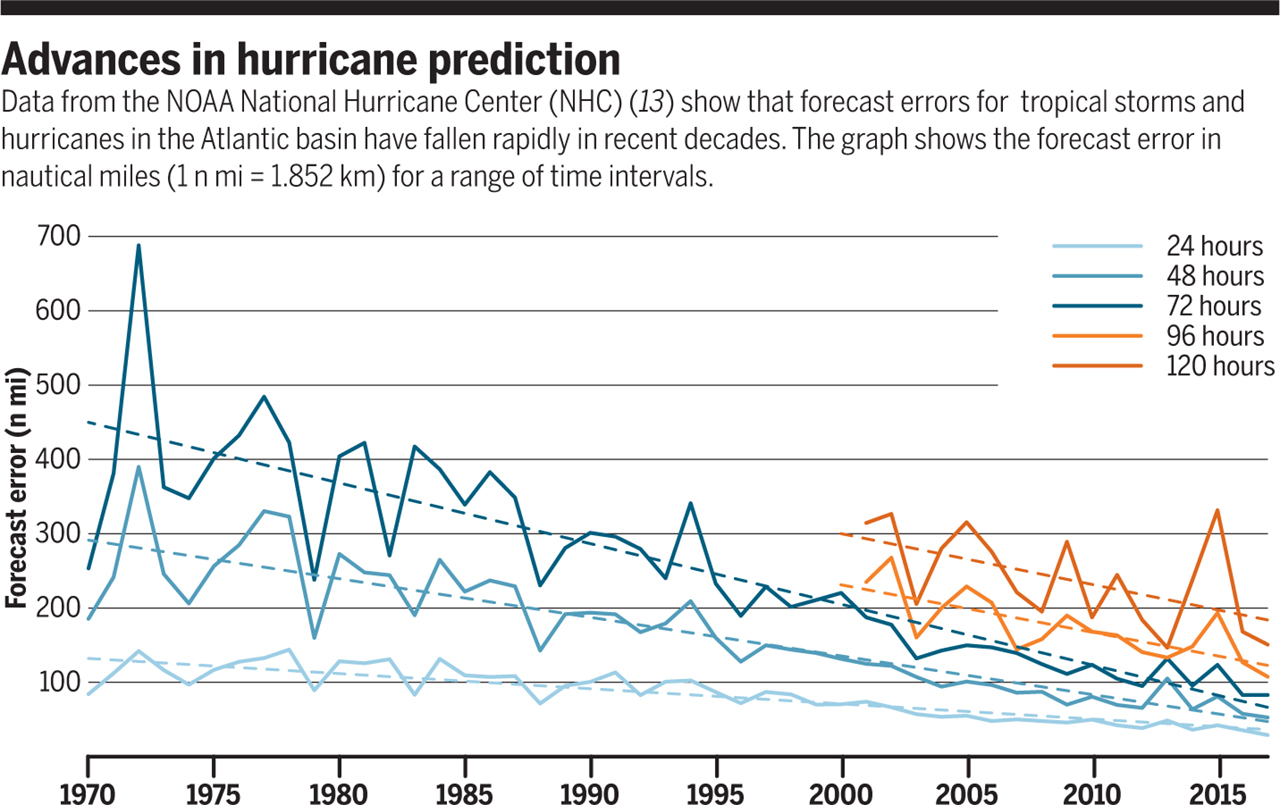
\includegraphics[width = 0.8\textwidth]{figures/alley_advances_2019_fig2}
\end{center}

\vfill
This is impressive. Source: Alley et al 2019

\end{frame}
%%%%%%%%%%%%%%%%%%%%%%%%%%%%%
\begin{frame}

The following conditions make prediction easier for weather than many of the others domains we have studied in the past:
\begin{itemize}
\item Many groups make public predictions every day at multiple time scales (5-day forecast, 10-day forecast), and we can all see how accurate they are
\pause
\item No self-fulfilling or self-defeating processes 
\pause
\item No concerns about causality
\pause
\item Predictions based a real physical model
\pause
\item Business and governments invests in improved performance
\end{itemize}

So even though this system is fundamentally unpredictable it has a lot going for it.
\end{frame}
%%%%%%%%%%%%%%%%%%%%%%%%%%%%%
\begin{frame}

They don't give up despite unpredictability.  Here are 4 key ideas that we might learn from them.

\end{frame}
%%%%%%%%%%%%%%%%%%%%%%%%%%%%
\begin{frame}

Parameterization: we don't have to model all sub-systems to include their impacts.

\pause
\begin{center}
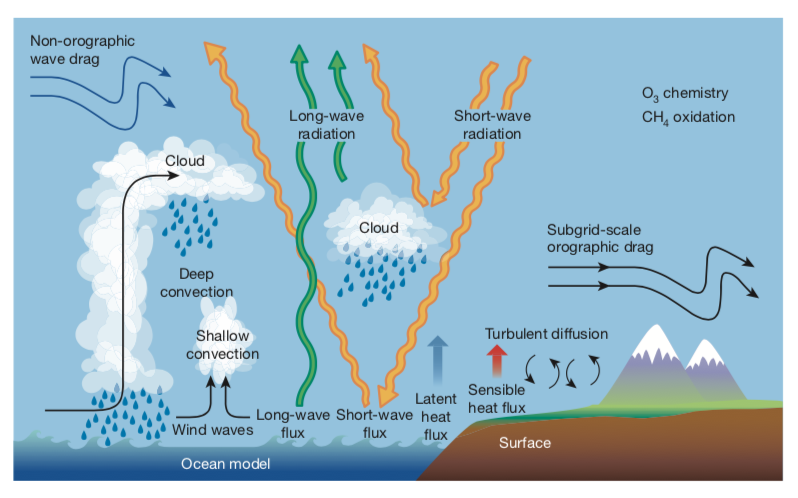
\includegraphics[width = 0.7\textwidth]{figures/bauer_quiet_2015_fig2}
\end{center}

\vfill
Example: multiple systems impacting the spread of COVID

\end{frame}
%%%%%%%%%%%%%%%%%%%%%%%%%%%%%
\begin{frame}

Ensemble forecasting: we want to average over many models and many initial conditions.

\begin{center}
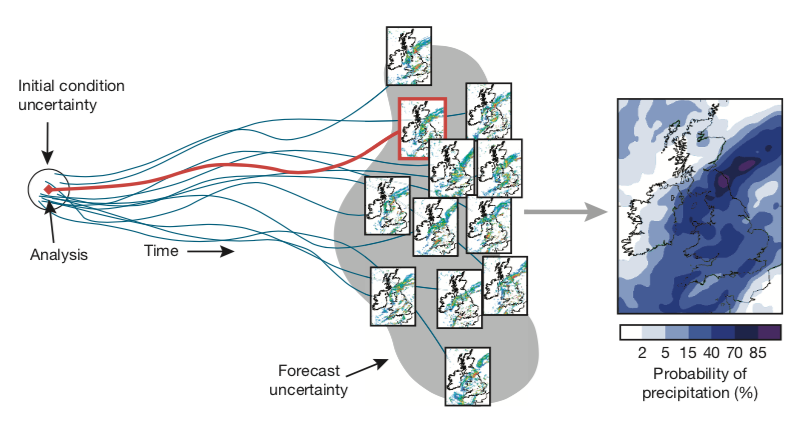
\includegraphics[width = 0.7\textwidth]{figures/bauer_quiet_2015_fig3}
\end{center}

\vfill
Example: pre-trial risk assessment 

\end{frame}
%%%%%%%%%%%%%%%%%%%%%%%%%%%%%
\begin{frame}

Model initialization is key (not just measuring the outcome)
\begin{center}
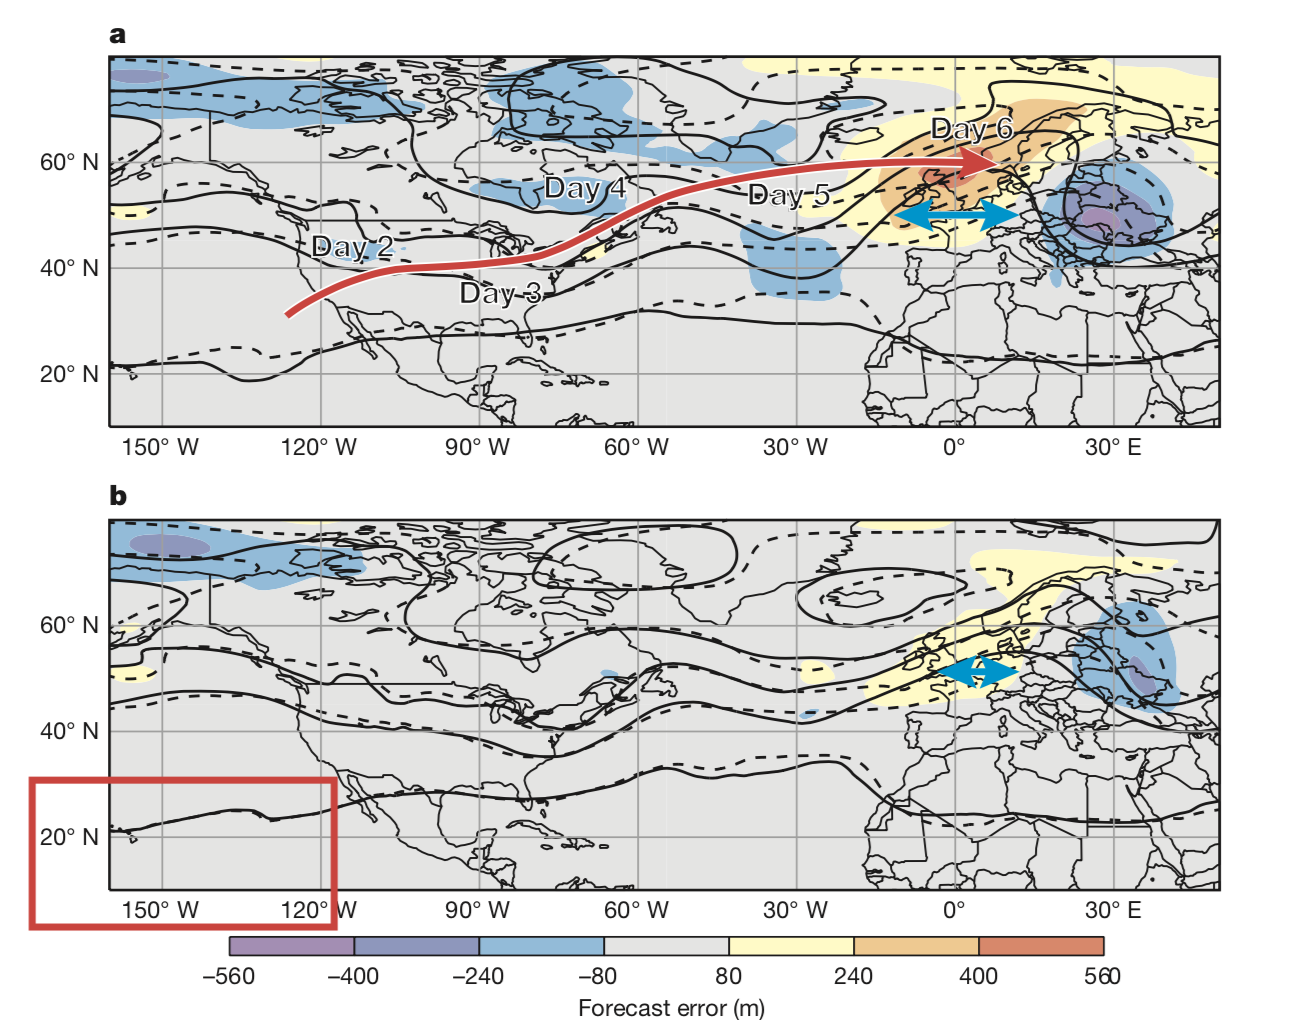
\includegraphics[width = 0.5\textwidth]{figures/bauer_quiet_2015_box1}
\end{center}

\vfill
\begin{itemize}
\item Contrast with Tetlock and Canadian CIA where we just focused on measuring the outcome
\pause
\item Crudely, errors come from two places: 1) model equations don't match true atmospheric equations, 2) bad initial conditions.
\end{itemize}

\end{frame}
%%%%%%%%%%%%%%%%%%%%%%%%%%%%
\begin{frame}

Massive global cooperation
\begin{center}

\includegraphics[width = 0.2\textwidth]{figures/wmo_logo}
\end{center}

\vfill
Contrast with the scale we normally work at in sociology

\end{frame}
%%%%%%%%%%%%%%%%%%%%%%%%%%%
\begin{frame}

4 key ideas that we might learn from them
\begin{itemize}
\item parameterization
\item ensemble forecasting
\item model initialization
\item massive global cooperation
\end{itemize}

\end{frame}
%%%%%%%%%%%%%%%%%%%%%
\begin{frame}

\begin{center}
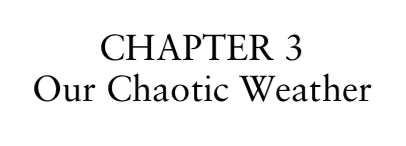
\includegraphics[width = 0.9\textwidth]{figures/lorenz_essence_1993_ch3}
\end{center}

\end{frame}
%%%%%%%%%%%%%%%%%%%%%%%%%%%%%
\begin{frame}
\frametitle{Idea 1}

\begin{itemize}
\item Forecasting tides: we are trying to predict the highly predictable regular response. 
\pause
\item Forecasting weather: we are trying to predict things beyond the highly predictable regular response (e.g., summer is warmer than winter)
\end{itemize}
\pause 
\vfill

\begin{itemize}
\item Might this be related to simple vs complex models? 
\pause
\item This reminds me of the question of whether we care about absolute prediction accuracy or prediction accuracy improvement relative to some benchmark
\pause
\item When do we want to oceanographers and when do we want to be meteorologists?
\end{itemize}

\end{frame}
%%%%%%%%%%%%%%%%%%%%
\begin{frame}
\frametitle{Idea 2}

The unperformable experiment: Change one atmosphere and leave another atmosphere unchanged, see how they diverge. Alternatives
\begin{itemize}
\item Look for twins
\end{itemize}

\end{frame}
%%%%%%%%%%%%%%%%%%%%%
\begin{frame}
\frametitle{Idea 2}

\begin{columns}[c]
  \column{.5\textwidth}
\begin{center}
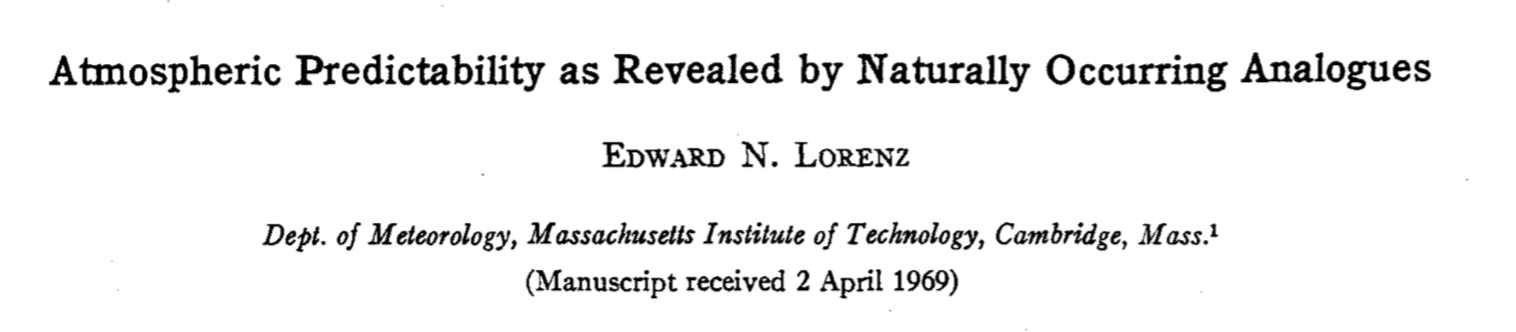
\includegraphics[width = 0.9\textwidth]{figures/lorenz_atmospheric_1969_title}
\end{center}
   \column{.5\textwidth} \pause
    \begin{center}
\begin{center}
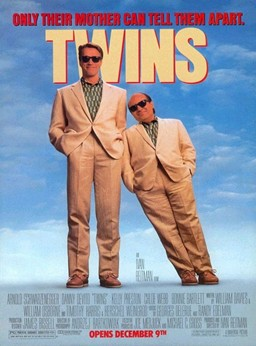
\includegraphics[height = 0.5\textheight]{figures/twins_poster}
\end{center}
    \end{center}
\end{columns}

\end{frame}
%%%%%%%%%%%%%%%%%%%%%
\begin{frame}
\frametitle{Idea 2}

The unperformable experiment: Change one atmosphere and leave another atmosphere unchanged, see how they diverge. Alternatives
\begin{itemize}
\item Look for twins
\pause
\item Physical models (dishpans)
\pause
\item Computer simulations of mathematical models \pause (To be continued . . . )
\end{itemize}

\end{frame}
%%%%%%%%%%%%%%%%%%%%%
\begin{frame}
\frametitle{Idea 3}

Global Atmospheric Research Program (GARP). Goal/selling point:
\begin{itemize}
\item Produce accurate two-week forecast
\pause
\item Pivot to determining whether such forecasts is feasible
\end{itemize}
\pause
\vfill
What if we made that switch for other problems?

\end{frame}
%%%%%%%%%%%%%%%%%%%%
\begin{frame}
\frametitle{Idea 4}

Even in a chaotic atmosphere some things are predictable (winds at high level in equatorial region)

\begin{center}
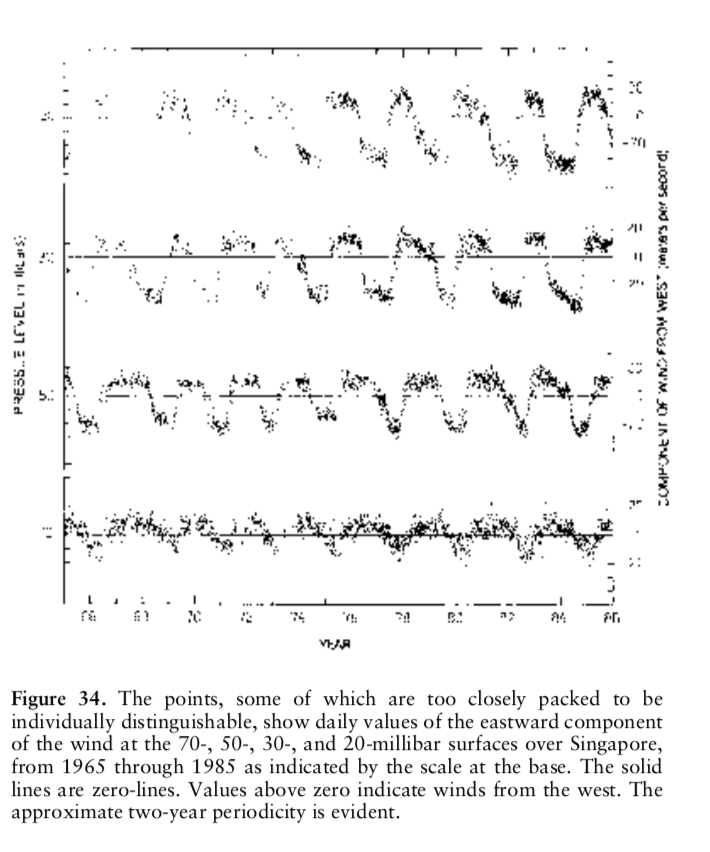
\includegraphics[width = 0.4\textwidth]{figures/lorenz_essence_1993_fig34_wcaption}
\end{center}

\vfill
Within systems that now appear unpredictable, are there parts that are predictable?

\end{frame}
%%%%%%%%%%%%%%%%%%%%
\begin{frame}

Four points:
\begin{itemize}
\item Sometimes we want to predict the typical outcome and when do we want to do better than predict the typical outcome
\pause
\item Even if we can't perform the experiment we want, we can use alternatives (twins, physical models, computer simulation of mathematical models)
\pause
\item Sometimes we want to make accurate predictions and sometimes we should study whether accurate predictions are possible
\pause
\item Even in a chaotic atmosphere some things are predictable (winds at high level in equatorial region)
\end{itemize}

\end{frame}
%%%%%%%%%%%%%%%%%%%%%%%%%%%
\begin{frame}

\begin{center}
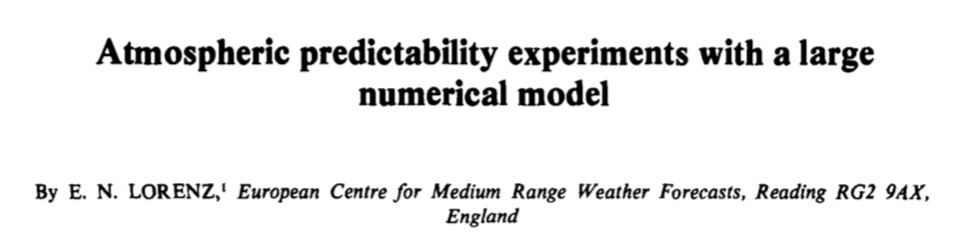
\includegraphics[width = 0.9\textwidth]{figures/lorenz_atmospheric_1982_title}
\end{center}

\vfill
Upper and lower bound on predictability with no extra computing!  

\end{frame}
%%%%%%%%%%%%%%%%%%%%%%%%%%%%%
\begin{frame}
\frametitle{}

We want to understand the upper bound and lower bound for accuracy using the model from the European Center for Medium Range Weather Forecasts (ECMWF) 
\begin{itemize}
\item How accurate are predictions?  This gives lower bound on accuracy.
\pause
\item How much do two similar initial conditions diverge?  This gives an upper bound on accuracy.
\end{itemize}


We'd like to do this without running the model many times because running the model is expensive.

\end{frame}
%%%%%%%%%%%%%%%%%%%%%%%%%%%%%
\begin{frame}
\frametitle{}

Model produces ``prognoses'':
\begin{itemize}
\item 1 Dec: 0 day, 1 day, 2 days $\ldots$, 10 days
\item 2 Dec: 0 day, 1 day, 2 days $\ldots$, 10 days
\item 3 Dec: 0 day, 1 day, 2 days $\ldots$, 10 days
\item $\vdots$
\item 10 March: 0 day, 1 day, 2 days $\ldots$, 10 days
\end{itemize}
\end{frame}
%%%%%%%%%%%%%%%%%%%%%%%%%%%%%
\begin{frame}
\frametitle{}

\begin{itemize}
\item 1 Dec: 0 day (1 Dec), 1 day (2 Dec), 2 days (3 Dec) $\ldots$, 10 days (11 Dec)
\pause
\item 2 Dec: 0 day (2 Dec), 1 day (3 Dec), 2 days (4 Dec) $\ldots$, 10 days (12 Dec)
\pause
\item 3 Dec: 0 day (3 Dec), 1 day (4 Dec), 2 days (5 Dec) $\ldots$, 10 days (13 Dec)
\pause
\item 4 Dec: 0 day (4 Dec), 1 day (5 Dec), 2 days (6 Dec) $\ldots$, 10 days (14 Dec)
\item $\vdots$
\end{itemize}

\end{frame}
%%%%%%%%%%%%%%%%%%%%%%%%%%%%%
\begin{frame}
\frametitle{}

How accurate are 1 day forecasts? This is equivalent to asking:  What is $E_{01}$?
\begin{itemize}
\item 1 Dec: 0 day (1 Dec), \textcolor{blue}{1 day (2 Dec)}, 2 days (3 Dec) $\ldots$, 10 days (11 Dec)
\item 2 Dec: \textcolor{blue}{0 day (2 Dec)}, 1 day (3 Dec), 2 days (4 Dec) $\ldots$, 10 days (12 Dec)
\item 3 Dec: 0 day (3 Dec), 1 day (4 Dec), 2 days (5 Dec) $\ldots$, 10 days (13 Dec)
\item 4 Dec: 0 day (4 Dec), 1 day (5 Dec), 2 days (6 Dec) $\ldots$, 10 days (14 Dec)
\item $\vdots$
\end{itemize}

\end{frame}
%%%%%%%%%%%%%%%%%%%%%%%%%%%%%
\begin{frame}
\frametitle{}

How accurate are 1 day forecasts? This is equivalent to asking:  What is $E_{01}$?
\begin{itemize}
\item 1 Dec: 0 day (1 Dec), 1 day (2 Dec), 2 days (3 Dec) $\ldots$, 10 days (11 Dec)
\item 2 Dec: 0 day (2 Dec), \textcolor{blue}{1 day (3 Dec)}, 2 days (4 Dec) $\ldots$, 10 days (12 Dec)
\item 3 Dec: \textcolor{blue}{0 day (3 Dec)}, 1 day (4 Dec), 2 days (5 Dec) $\ldots$, 10 days (13 Dec)
\item 4 Dec: 0 day (4 Dec), 1 day (5 Dec), 2 days (6 Dec) $\ldots$, 10 days (14 Dec)
\item $\vdots$
\end{itemize}

\end{frame}
%%%%%%%%%%%%%%%%%%%%%%%%%%%%%
\begin{frame}
\frametitle{}

How accurate are 2 day forecasts? This is equivalent to asking:  What is $E_{02}$?
\begin{itemize}
\item 1 Dec: 0 day (1 Dec), 1 day (2 Dec), \textcolor{blue}{2 days (3 Dec)} $\ldots$, 10 days (11 Dec)
\item 2 Dec: 0 day (2 Dec), 1 day (3 Dec), 2 days (4 Dec) $\ldots$, 10 days (12 Dec)
\item 3 Dec: \textcolor{blue}{0 day (3 Dec)}, 1 day (4 Dec), 2 days (5 Dec) $\ldots$, 10 days (13 Dec)
\item 4 Dec: 0 day (4 Dec), 1 day (5 Dec), 2 days (6 Dec) $\ldots$, 10 days (14 Dec)
\item $\vdots$
\end{itemize}

\end{frame}
%%%%%%%%%%%%%%%%%%%%%%%%%%%%%
\begin{frame}
\frametitle{}

How accurate are 2 day forecasts? This is equivalent to asking:  What is $E_{02}$?
\begin{itemize}
\item 1 Dec: 0 day (1 Dec), 1 day (2 Dec), 2 days (3 Dec) $\ldots$, 10 days (11 Dec)
\item 2 Dec: 0 day (2 Dec), 1 day (3 Dec), \textcolor{blue}{2 days (4 Dec)} $\ldots$, 10 days (12 Dec)
\item 3 Dec: 0 day (3 Dec), 1 day (4 Dec), 2 days (5 Dec) $\ldots$, 10 days (13 Dec)
\item 4 Dec: \textcolor{blue}{0 day (4 Dec)}, 1 day (5 Dec), 2 days (6 Dec) $\ldots$, 10 days (14 Dec)
\item $\vdots$
\end{itemize}

\end{frame}
%%%%%%%%%%%%%%%%%%%%%%%%%%%%%
\begin{frame}

\begin{center}
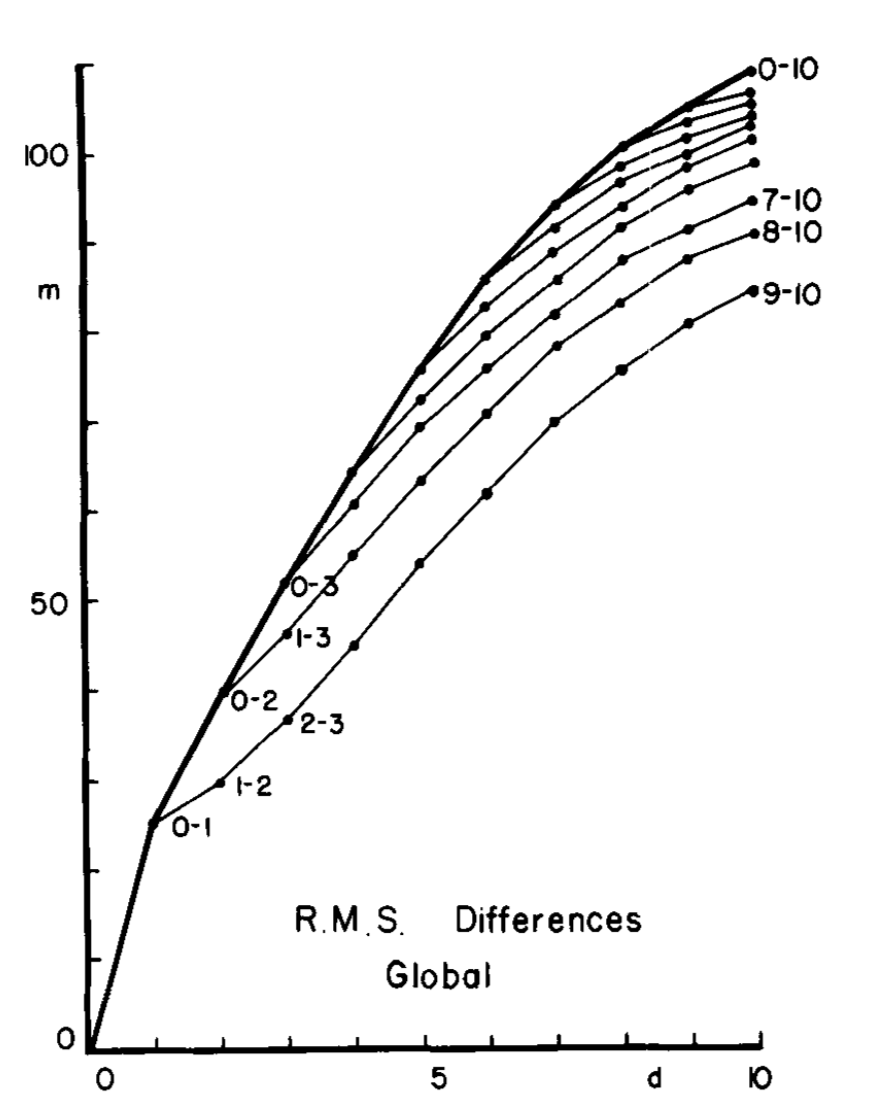
\includegraphics[height = 0.8\textheight]{figures/lorenz_atmospheric_1982_fig1}
\end{center}

\vfill
$E_{01}, E_{02}, \ldots E_{010}$ is the heavy curve at the top

\end{frame}
%%%%%%%%%%%%%%%%%%%%%%%%%%%%%
\begin{frame}

What about two trajectories that start close together?  How fast do they diverge?

\end{frame}
%%%%%%%%%%%%%%%%%%%%%%%%%%%%%
\begin{frame}
\frametitle{}

\begin{itemize}
\item 1 Dec: 0 day (1 Dec), \textcolor{red}{1 day (2 Dec)}, \textcolor{blue}{2 days (3 Dec)} $\ldots$
\item 2 Dec: \textcolor{red}{0 day (2 Dec)}, \textcolor{blue}{1 day (3 Dec)}, 2 days (4 Dec) $\ldots$
\item 3 Dec: 0 day (3 Dec), 1 day (4 Dec), 2 days (5 Dec) $\ldots$ 
\item 4 Dec: 0 day (4 Dec), 1 day (5 Dec), 2 days (6 Dec) $\ldots$
\item $\vdots$
\end{itemize}

\pause

\vfill
Distance between \textcolor{red}{0 day (2 Dec)} and \textcolor{red}{1 day (2 Dec)}: $\epsilon$\\
\pause
Distance between \textcolor{blue}{1 day (3 Dec)} and  \textcolor{blue}{2 days (3 Dec)}: $c \cdot \epsilon$ for $(c > 1)$

\end{frame}
%%%%%%%%%%%%%%%%%%%%%%%%%%%%%
\begin{frame}
\frametitle{}

\begin{itemize}
\item 1 Dec: 0 day (1 Dec), 1 day (2 Dec), 2 days (3 Dec) $\ldots$
\item 2 Dec: 0 day (2 Dec), \textcolor{red}{1 day (3 Dec)}, \textcolor{blue}{2 days (4 Dec)} $\ldots$
\item 3 Dec: \textcolor{red}{0 day (3 Dec)}, \textcolor{blue}{1 day (4 Dec)}, 2 days (5 Dec) $\ldots$
\item 4 Dec: 0 day (4 Dec), 1 day (5 Dec), 2 days (6 Dec) $\ldots$
\item $\vdots$
\end{itemize}

\pause
\vfill
\onslide<2->{Distance between \textcolor{red}{0 day (3 Dec)} and \textcolor{red}{1 day (3 Dec)}: $\epsilon$} \onslide<4->{$(E_{01})$} \\
\onslide<3->{Distance between \textcolor{blue}{1 day (4 Dec)} and \textcolor{blue}{2 days (4 Dec)}: $c \cdot \epsilon$ for $(c > 1)$} \onslide<5->{$(E_{12})$}

\end{frame}
%%%%%%%%%%%%%%%%%%%%%%%%%%%%%
\begin{frame}
\frametitle{}

\begin{itemize}
\item 1 Dec: 0 day (1 Dec), 1 day (2 Dec), 2 days (3 Dec), 3 days (4 Dec) $\ldots$
\item 2 Dec: 0 day (2 Dec), \textcolor{red}{1 day (3 Dec)}, 2 days (4 Dec), \textcolor{blue}{3 days (5 Dec)} $\ldots$
\item 3 Dec: \textcolor{red}{0 day (3 Dec)}, 1 day (4 Dec), \textcolor{blue}{2 days (5 Dec)} 3 days (6 Dec) $\ldots$
\item 4 Dec: 0 day (4 Dec), 1 day (5 Dec), 2 days (6 Dec), 3 days (7 Dec) $\ldots$
\item $\vdots$
\end{itemize}

\pause
\vfill
\onslide<2->{Distance between \textcolor{red}{0 day (3 Dec)} and \textcolor{red}{1 day (3 Dec)}: $\epsilon$} \onslide<4->{$(E_{01})$} \\
\onslide<3->{Distance between \textcolor{blue}{2 day (5 Dec)} and \textcolor{blue}{3 days (5 Dec)}: $c \cdot \epsilon$ for $(c > 1)$} \onslide<5->{$(E_{23})$}

\end{frame}
%%%%%%%%%%%%%%%%%%%%%%%%%%%%%
\begin{frame}

\begin{center}
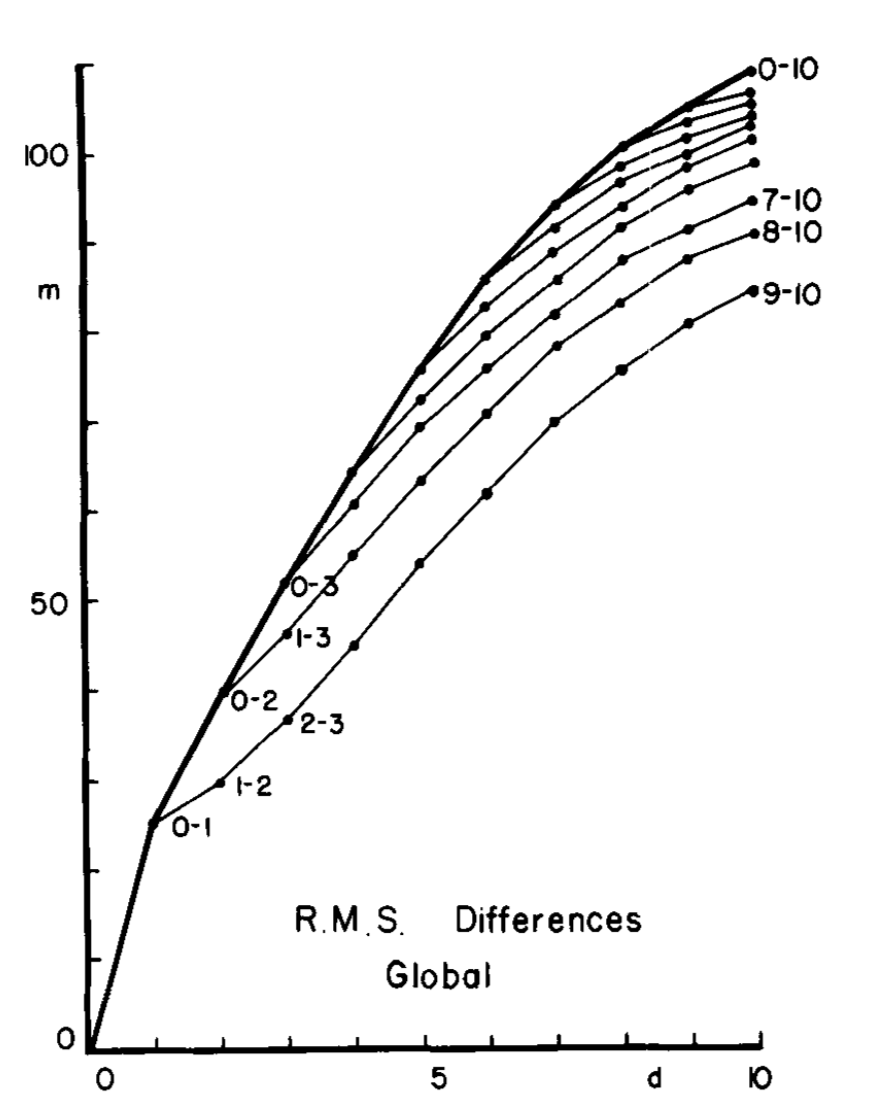
\includegraphics[height = 0.8\textheight]{figures/lorenz_atmospheric_1982_fig1}
\end{center}

\vfill
$E_{12}, E_{23}, \ldots E_{910}$ is the light curve at the bottom

\end{frame}
%%%%%%%%%%%%%%%%%%%%%%%%%%%%%
\begin{frame}

\onslide<1>{What about two trajectories that start close together?  How fast do they diverge?}\\
\onslide<2->{\sout{What about two trajectories that start close together?  How fast do they diverge?}}
\onslide<2->{What about two trajectories that start a bit further apart?  How fast do they diverge?}

\end{frame}
%%%%%%%%%%%%%%%%%%%%%%%%%%%%%
\begin{frame}
\frametitle{}

\small{
\begin{itemize}
\item 1 Dec: 0 day (1 Dec), 1 day (2 Dec), \textcolor{red}{2 days (3 Dec)}, \textcolor{blue}{3 days (4 Dec)}, 4 days (5 Dec) $\ldots$
\item 2 Dec: 0 day (2 Dec), 1 day (3 Dec), 2 days (4 Dec), 3 days (5 Dec), 4 days (6 Dec) $\ldots$
\item 3 Dec: \textcolor{red}{0 day (3 Dec)}, \textcolor{blue}{1 day (4 Dec)}, 2 days (5 Dec), 3 days (6 Dec), 4 days (7 Dec) $\ldots$
\item 4 Dec: 0 day (4 Dec), 1 day (5 Dec), 2 days (6 Dec), 3 days (7 Dec), 4 days (8 Dec) $\ldots$
\item $\vdots$
\end{itemize}
}

\vfill

\onslide<2->{Distance between \textcolor{red}{0 day (3 Dec)} and \textcolor{red}{2 day (3 Dec)}: $\epsilon$} \onslide<4->{$(E_{02})$} \\
\onslide<3->{Distance between \textcolor{blue}{1 day (4 Dec)} and \textcolor{blue}{3 days (4 Dec)}: $c \cdot \epsilon$ for $(c > 1)$} \onslide<5->{$(E_{13})$}\\

\end{frame}
%%%%%%%%%%%%%%%%%%%%%%%%%%%%%
\begin{frame}
\frametitle{}

\small{
\begin{itemize}
\item 1 Dec: 0 day (1 Dec), 1 day (2 Dec), \textcolor{red}{2 days (3 Dec)}, 3 days (4 Dec), \textcolor{blue}{4 days (5 Dec)}  $\ldots$
\item 2 Dec: 0 day (2 Dec), 1 day (3 Dec), 2 days (4 Dec), 3 days (5 Dec), 4 days (6 Dec)  $\ldots$
\item 3 Dec: \textcolor{red}{0 day (3 Dec)}, 1 day (4 Dec), \textcolor{blue}{2 days (5 Dec)}, 3 days (6 Dec), 4 days (7 Dec) $\ldots$
\item 4 Dec: 0 day (4 Dec), 1 day (5 Dec), 2 days (6 Dec),  3 days (7 Dec), 4 days (8 Dec) $\ldots$
\item $\vdots$
\end{itemize}
}

\vfill
\onslide<2->{Distance between \textcolor{red}{0 day (3 Dec)} and \textcolor{red}{2 day (3 Dec)}: $\epsilon$} \onslide<4->{$(E_{02})$} \\
\onslide<3->{Distance between \textcolor{blue}{2 day (5 Dec)} and \textcolor{blue}{4 days (5 Dec)}: $c \cdot \epsilon$ for $(c > 1)$} \onslide<5->{$(E_{24})$}

\end{frame}
%%%%%%%%%%%%%%%%%%%%%%%%%%%%%
\begin{frame}

\begin{center}
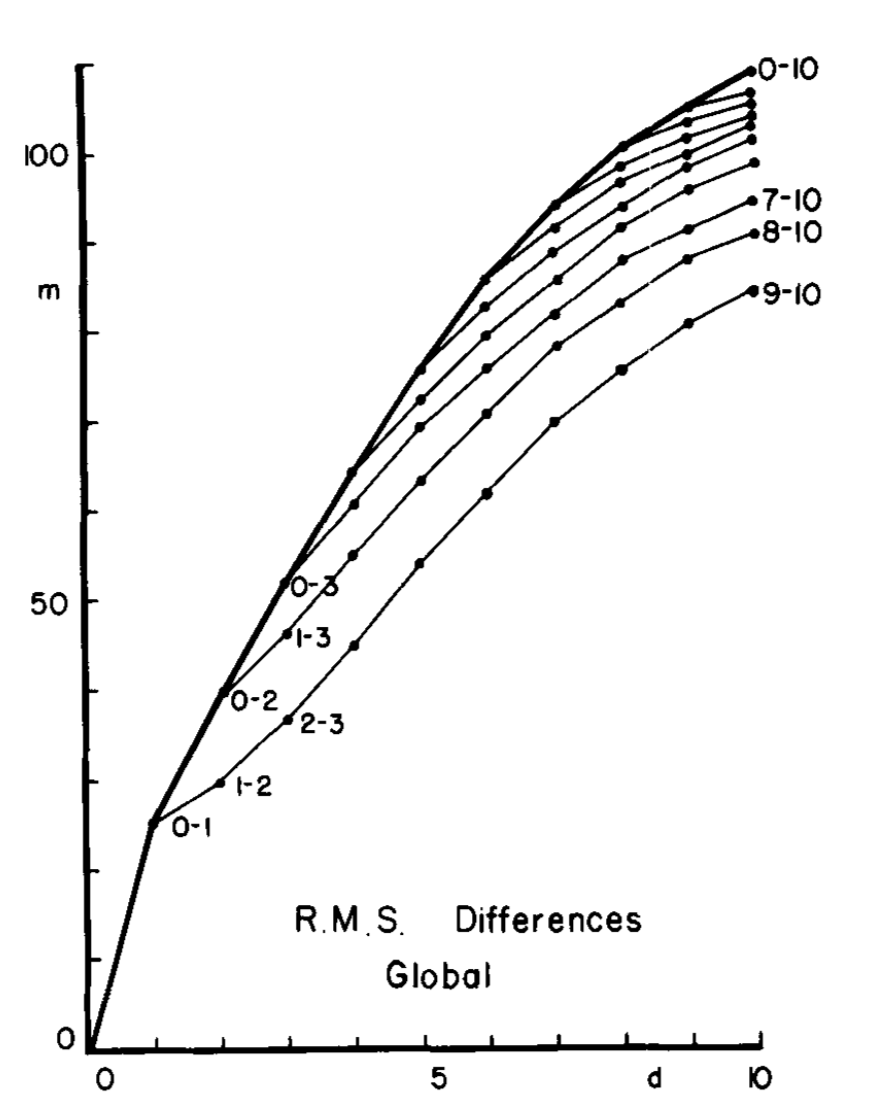
\includegraphics[height = 0.8\textheight]{figures/lorenz_atmospheric_1982_fig1}
\end{center}

\vfill
$E_{12}, E_{23}, \ldots E_{910}$ is the light curve second from the bottom

\end{frame}
%%%%%%%%%%%%%%%%%%%%%%%%%%%%%
\begin{frame}

\begin{center}
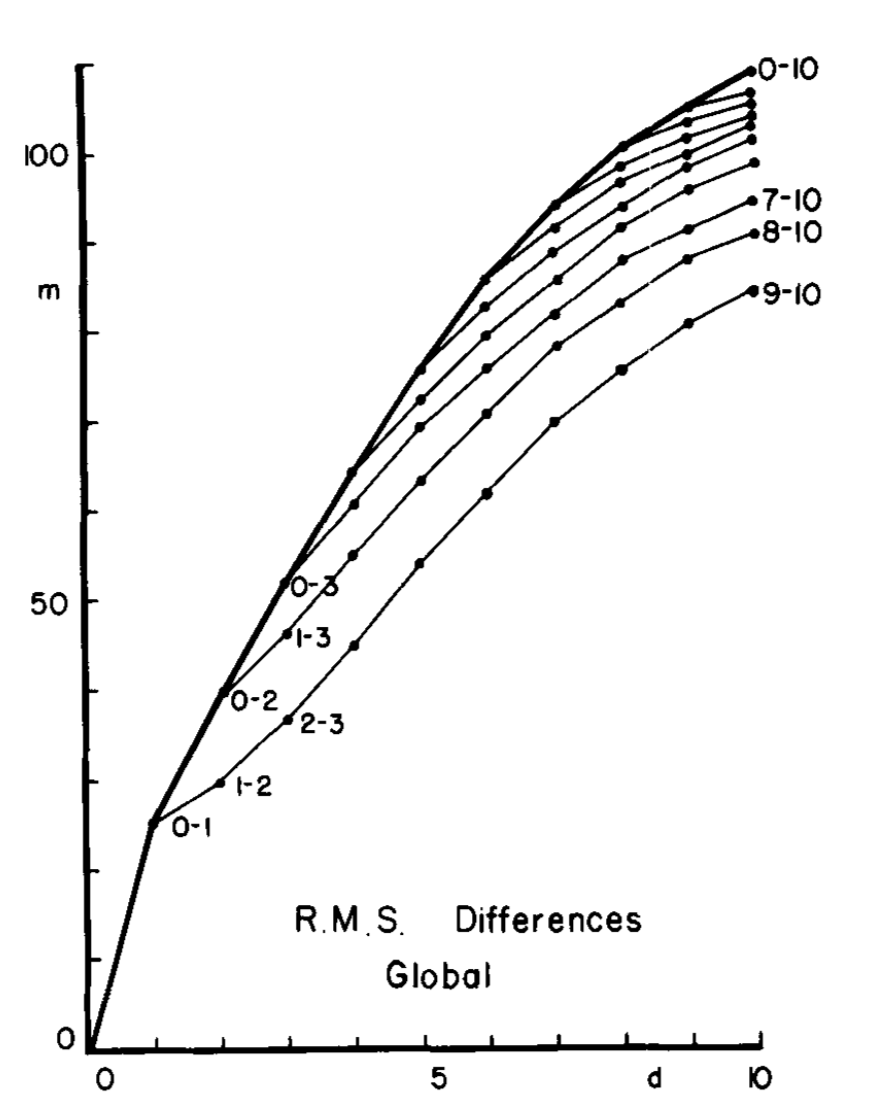
\includegraphics[height = 0.6\textheight]{figures/lorenz_atmospheric_1982_fig1}
\end{center}

\begin{itemize}
\item Heavy curve (top) compares two different equations: ``true'' atmosphere and ECMWF
\pause
\item Thin curves compare the same equations: ECMWF and ECMWF
\pause
\item ``The excess slope of the heavy curve over that of an intersection thin curve may therefore be regarded as a measure of the maximum amount by which the model may still be improved.''  \emph{Have you seen this anywhere else?}
\end{itemize}

\end{frame}
%%%%%%%%%%%%%%%%%%%%%%%%%%%%%
\begin{frame}

\begin{center}
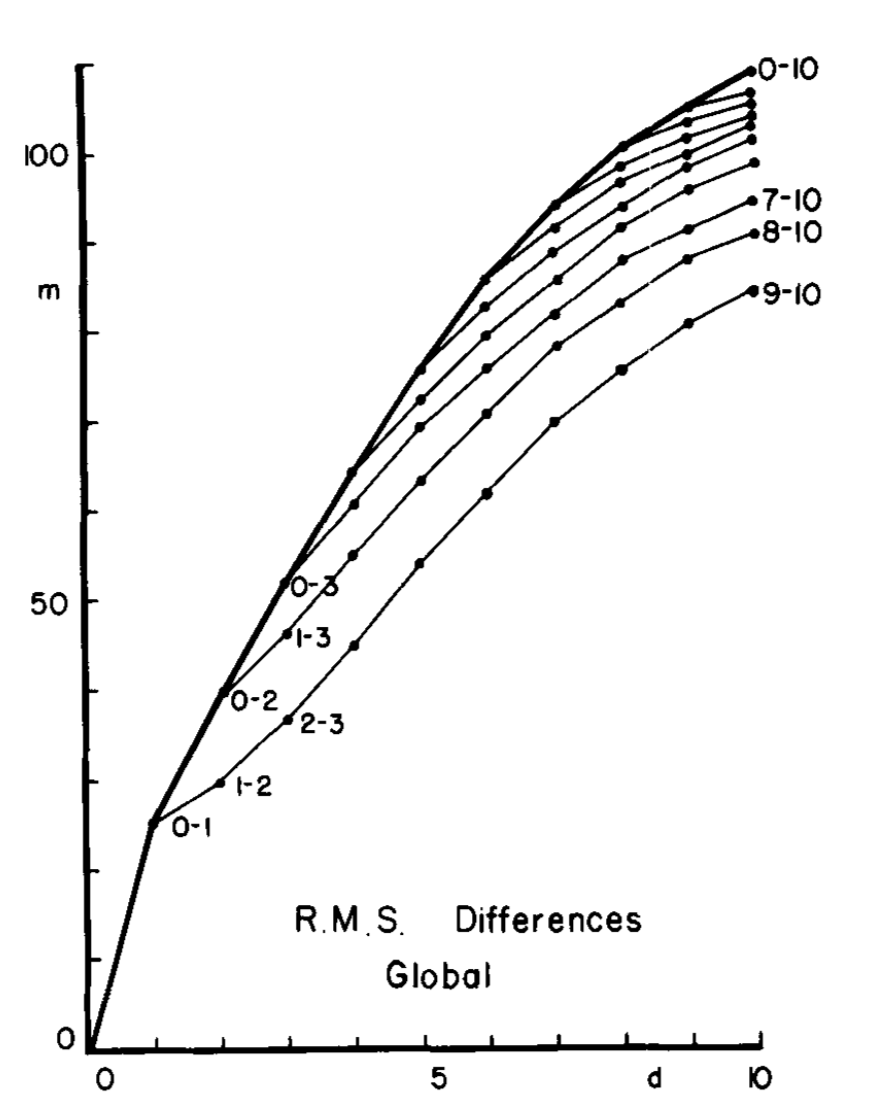
\includegraphics[height = 0.5\textheight]{figures/lorenz_atmospheric_1982_fig1}
\end{center}

\begin{itemize}
\item The curves should level off at the same value: RMS difference between two randomly chosen weathers (``analyses''), RMS difference between two randomly chosen forecasts (``prognoses'').  Call this leveling off point ``the ceiling''.
\pause
\item How quickly do we get to the ceiling?
\pause
\item $E_{01} = 25$ which takes about 3.5 days to double. 
\pause
\item Under some assumptions, time for errors to go from $\frac{1}{3}$ to $\frac{1}{2}$ $=$ time from $\frac{1}{2}$ to $\frac{2}{3}$ $=$ the time that small errors double. Based on Fig 1, this is 2.5 days.
\end{itemize}

\end{frame}
%%%%%%%%%%%%%%%%%%%%%%%%%%%%%
\begin{frame}

What is the rate of change of the error ($dE/dt$) as a function of the error $(E)$?  This is related to how long it will take us to get to the ceiling.

\begin{columns}[c]
  \column{.5\textwidth}
\begin{center}
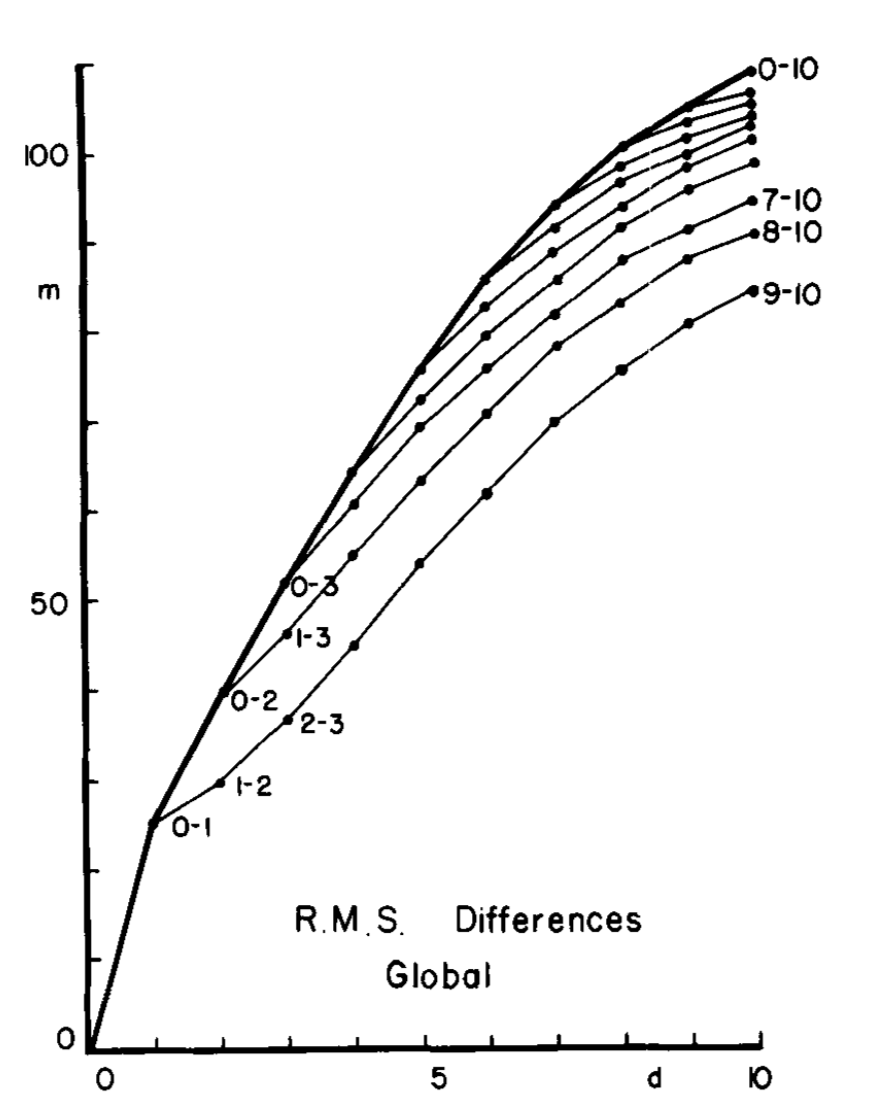
\includegraphics[height = 0.5\textheight]{figures/lorenz_atmospheric_1982_fig1}
\end{center}
   \column{.5\textwidth} \pause
    \begin{center}
\begin{center}
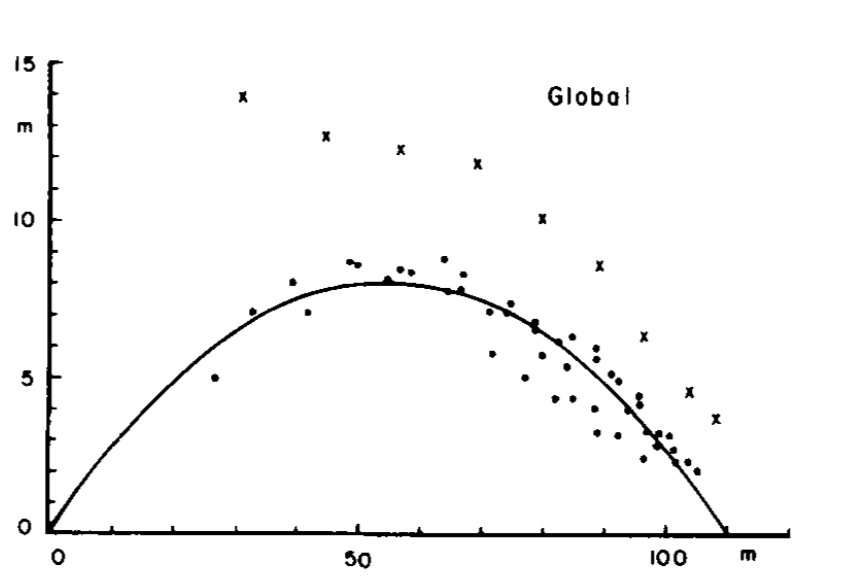
\includegraphics[height = 0.5\textheight]{figures/lorenz_atmospheric_1982_fig2}
\end{center}
    \end{center}
\end{columns}

\end{frame}
%%%%%%%%%%%%%%%%%%%%%%%%%%%%%
\begin{frame}

\begin{center}
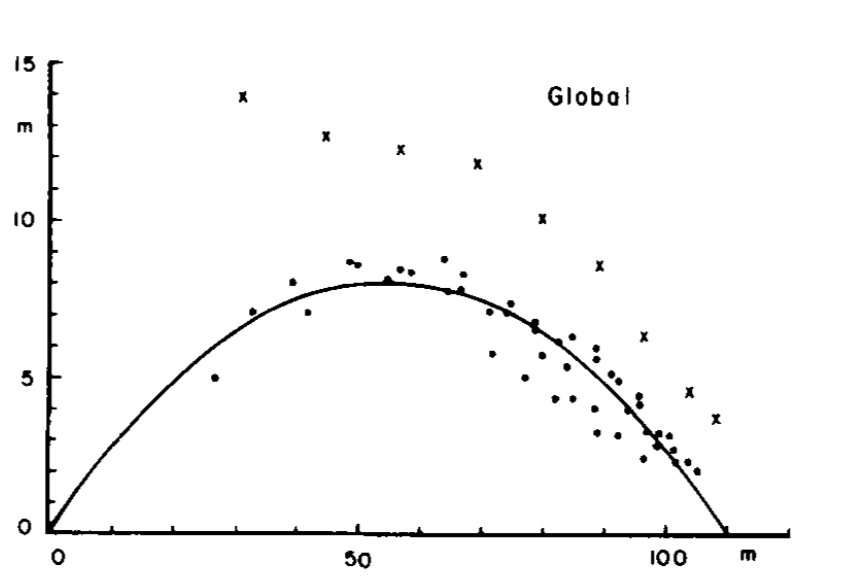
\includegraphics[height = 0.5\textheight]{figures/lorenz_atmospheric_1982_fig2}
\end{center}

\begin{itemize}
\item x-axis: error, y-axis: rate of growth of error
\pause
\item difference between crosses (prognosis vs analysis) and dots (prognosis vs prognosis) shows room for improvement in prognosis
\end{itemize}

\end{frame}
%%%%%%%%%%%%%%%%%%%%%%%%%%%%%
\begin{frame}

But are these improvements really possible? Yes, he shows in Sec 4 (the part I didn't assign)

\end{frame}
%%%%%%%%%%%%%%%%%%%%%%%%%%%%%
\begin{frame}

First, he does a post-hoc correction (kind of like numerical calibration) \pause
\begin{columns}[c]
  \column{.5\textwidth}
\begin{center}
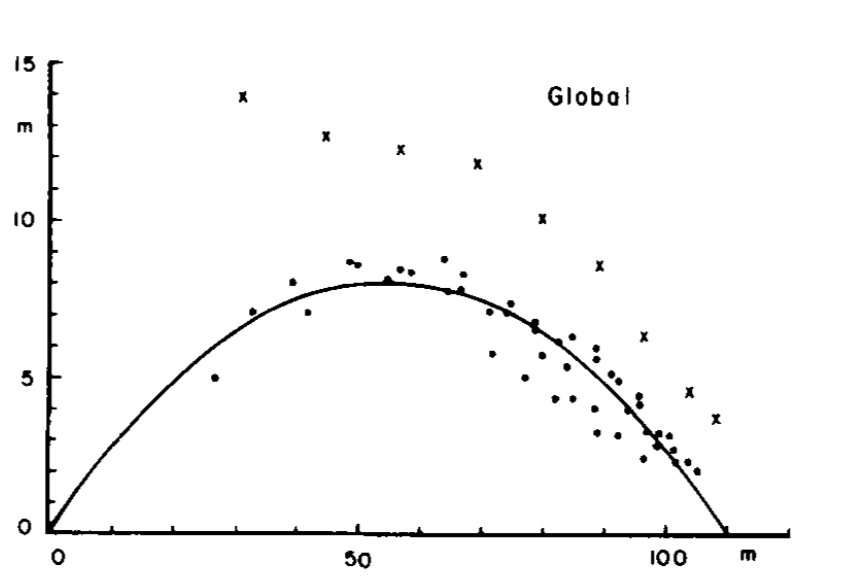
\includegraphics[height = 0.5\textheight]{figures/lorenz_atmospheric_1982_fig2}
Original
\end{center}
   \column{.5\textwidth} \pause
    \begin{center}
\begin{center}
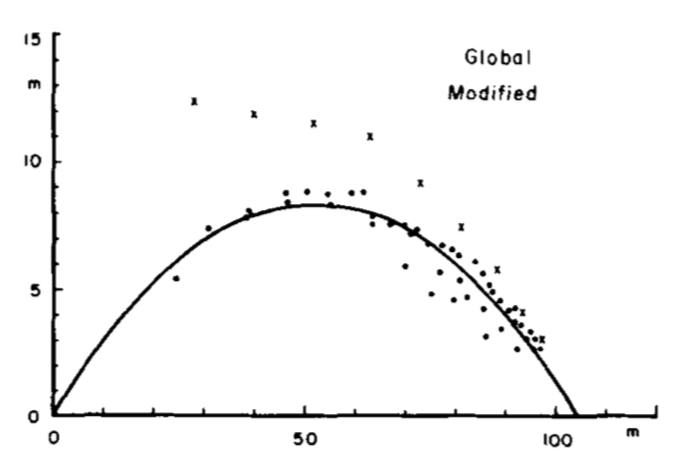
\includegraphics[height = 0.5\textheight]{figures/lorenz_atmospheric_1982_fig3}
``Calibrated''
\end{center}
    \end{center}
\end{columns}

\begin{itemize}
\item x-axis: error, y-axis: rate of growth of error
\pause
\item ``Calibrated'' prognoses make crosses closer to dots.
\pause
\item Improvements likely to come when errors are mid-sized not large
\end{itemize}

\end{frame}
%%%%%%%%%%%%%%%%%%%%%%%%%%%%
\begin{frame}

\begin{columns}[c]
  \column{.5\textwidth}
\begin{center}
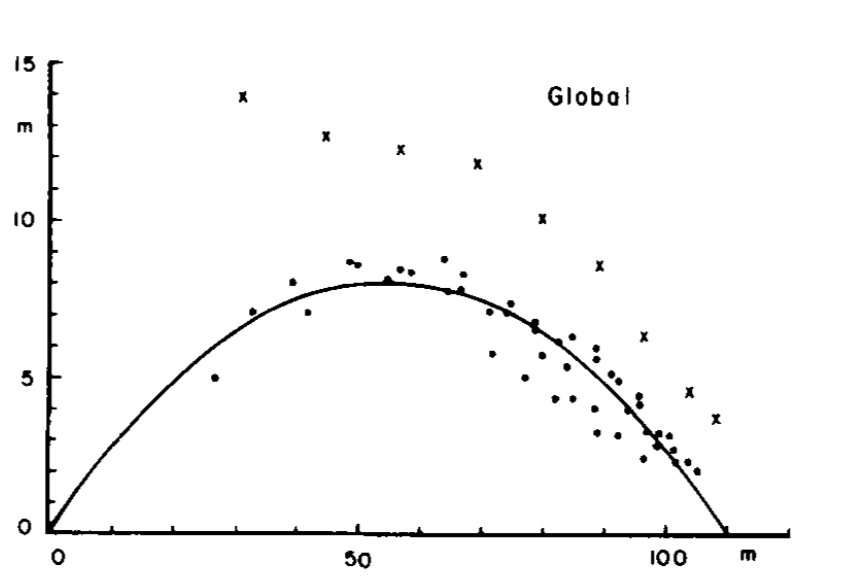
\includegraphics[height = 0.5\textheight]{figures/lorenz_atmospheric_1982_fig2}
Global
\end{center}
   \column{.5\textwidth} \pause
    \begin{center}
\begin{center}
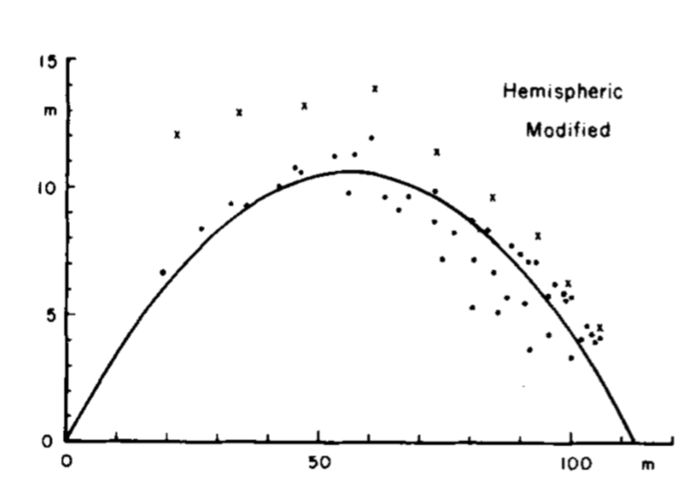
\includegraphics[height = 0.5\textheight]{figures/lorenz_atmospheric_1982_fig4}
Northern Hemisphere + ``Calibrated''
\end{center}
    \end{center}
\end{columns}

\begin{itemize}
\item x-axis: error, y-axis: rate of growth of error
\pause
\item In Norther Hemisphere difference between crosses (prognosis vs analysis) and dots (prognosis vs prognosis) is smaller
\end{itemize}

\end{frame}
%%%%%%%%%%%%%%%%%%%%%%%%%%%%%
\begin{frame}

\begin{center}
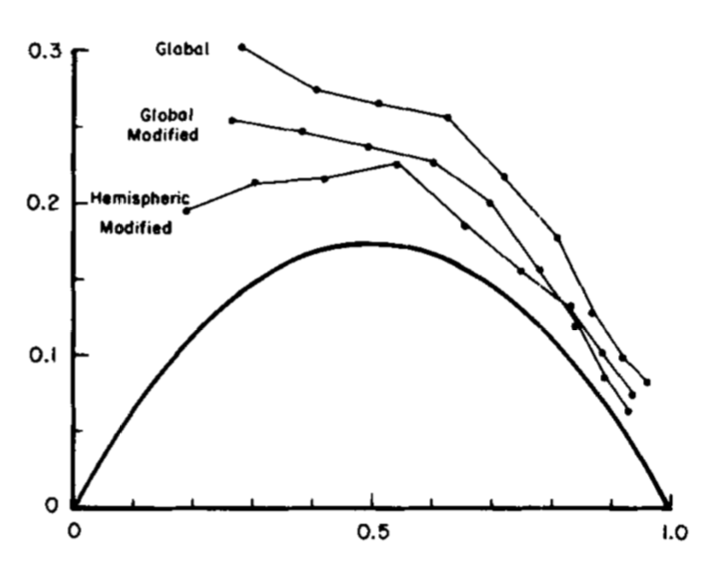
\includegraphics[height = 0.5\textheight]{figures/lorenz_atmospheric_1982_fig5}
\end{center}

\begin{itemize}
\item ``Accepting the modified ECMWF model, applied to the NH, as a state-of-the-art model, we find that we have established upper and lower bounds to atmospheric predictability which are reasonably close together.''
\pause
\item ``Assuming that we have correctly estimated the doubling time, we find that, even without further improvements in one-day forecasting, we may eventually make 10 day forecasts as good as present 7 day forecasts . . . .''
\end{itemize}

\end{frame}
%%%%%%%%%%%%%%%%%%%%%%%%%%%%%
\begin{frame}

``Assuming that we have correctly estimated the doubling time, we find that, even without further improvements in one-day forecasting, we may eventually make 10 day forecasts as good as present 7 day forecasts . . . .'' Lorenz 1982 \pause

\begin{center}
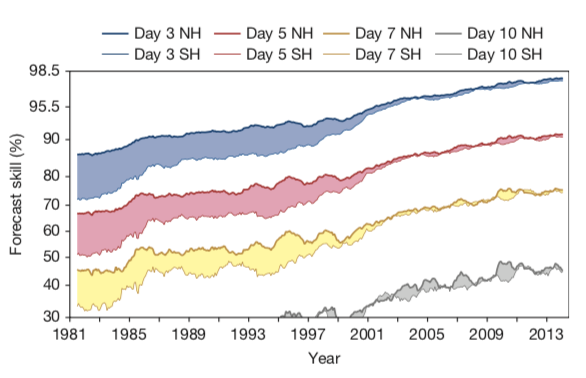
\includegraphics[width = 0.8\textwidth]{figures/bauer_quiet_2015_fig1}
\end{center}

\end{frame}
%%%%%%%%%%%%%%%%%%%%%%%%%%%%%%
\begin{frame}

``Assuming that we have correctly estimated the doubling time, we find that, even without further improvements in one-day forecasting, we may eventually make 10 day forecasts as good as present 7 day forecasts . . . .'' Lorenz 1982 \pause

\begin{center}
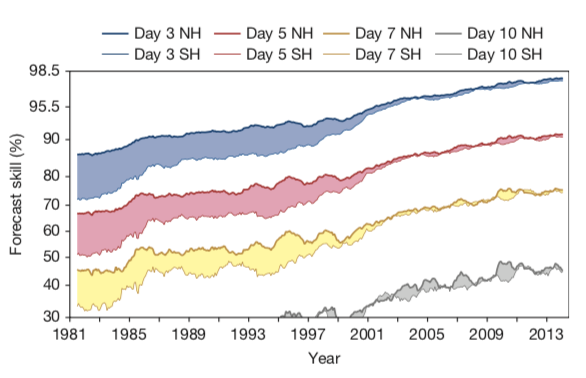
\includegraphics[width = 0.8\textwidth]{figures/bauer_quiet_2015_fig1}
\end{center}

\end{frame}
%%%%%%%%%%%%%%%%%%%%%%%%%%%%%%
\begin{frame}

\begin{center}
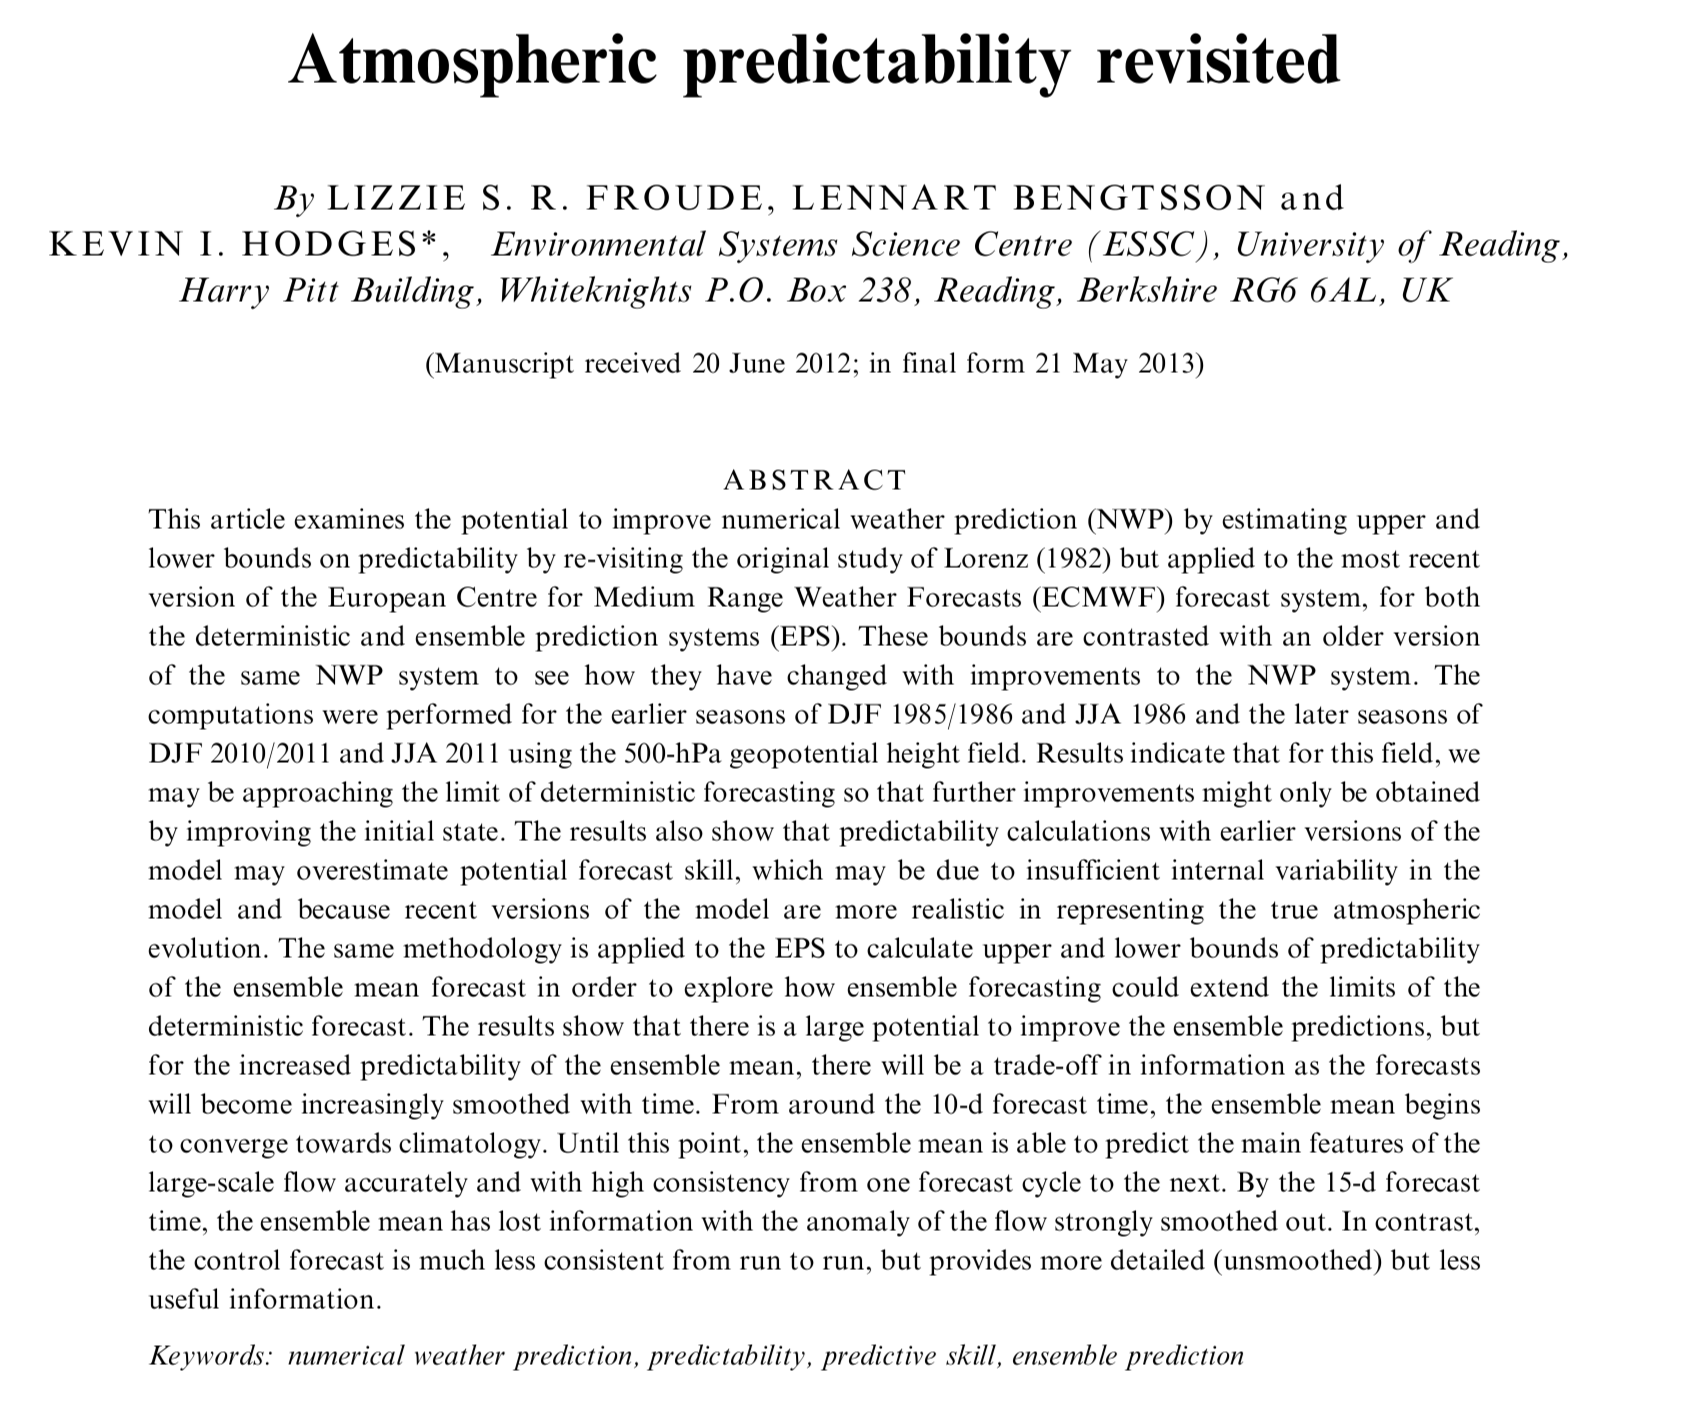
\includegraphics[width = 0.6\textwidth]{figures/froude_atmospheric_2013_title_abstract}
\end{center}

\end{frame}
%%%%%%%%%%%%%%%%%%%%%%%%%%%%%
\begin{frame}

\begin{center}
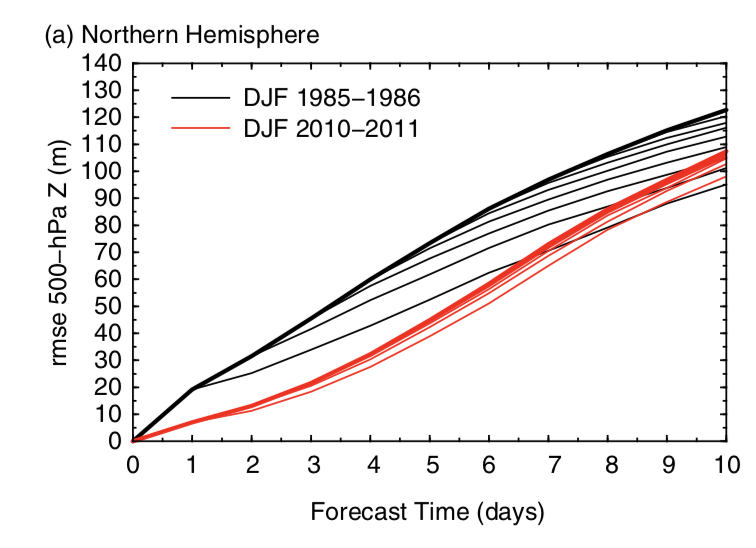
\includegraphics[width = 0.7\textwidth]{figures/froude_atmospheric_2013_fig2a}
\end{center}

\vfill
Note the compression between thick and think lines. DJF = Dec, Jan, Feb
\end{frame}
%%%%%%%%%%%%%%%%%%%%%%%%%%%%%%
\begin{frame}

\begin{center}
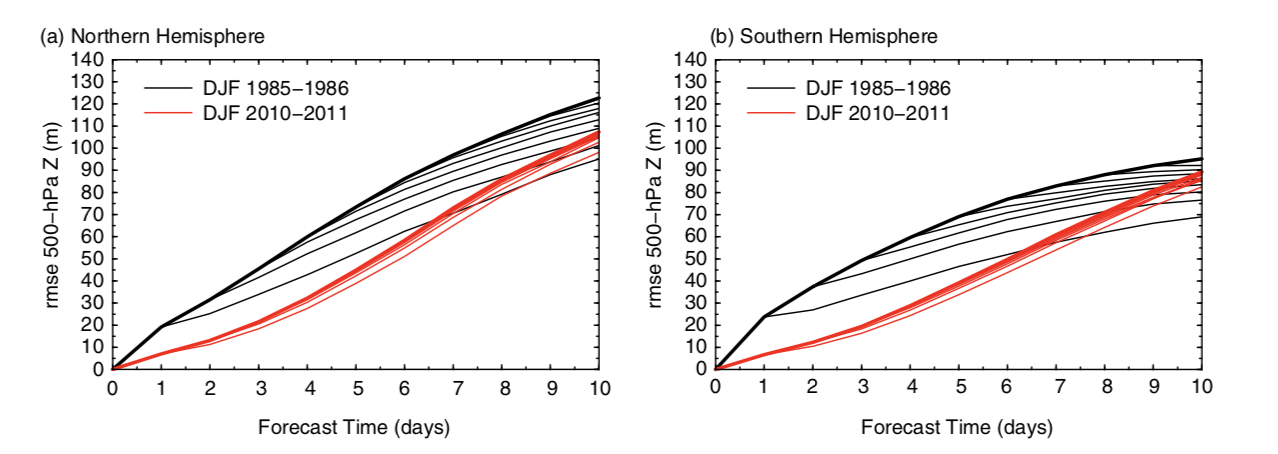
\includegraphics[width = 0.9\textwidth]{figures/froude_atmospheric_2013_fig2ab}
\end{center}

\vfill
\small{Note compression between thick and think lines. DJF = Dec, Jan, Feb}
\end{frame}
%%%%%%%%%%%%%%%%%%%%%%%%%%%%%%
\begin{frame}

\begin{center}
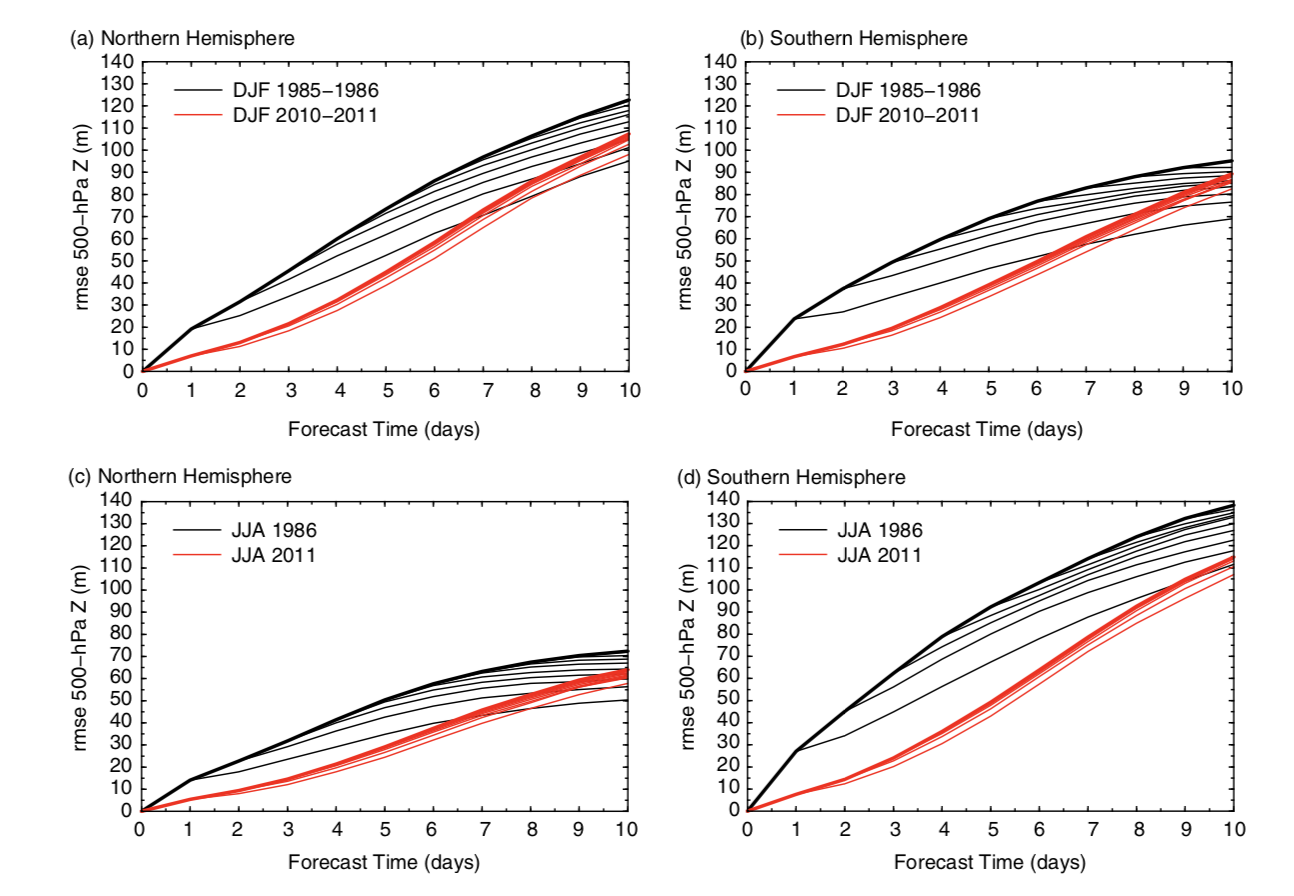
\includegraphics[width = 0.7\textwidth]{figures/froude_atmospheric_2013_fig2}
\end{center}

\vfill
\small{Note compression between thick and think lines. DJF = Dec, Jan, Feb; JJA = Jun, Jul, Aug}
\end{frame}
%%%%%%%%%%%%%%%%%%%%%%%%%%%%%%
\begin{frame}

Rough summary of insight from Lorenz (1982): by simulating weather we can learn how much weather simulation can be improved.   That seems surprising and potentially valuable.  This seems to require that we attempt to match our predictions to real data.

\end{frame}
%%%%%%%%%%%%%%%%%%%%%%%%%%%%%%
\begin{frame}

Stepping back

\end{frame}
%%%%%%%%%%%%%%%%%%%%%%%%%%%%%%
\begin{frame}

3 takeways
\begin{itemize}
\item It is possible to make long-term improvements in predictability so what we can do now is not the limit of what is possible (limitation of brute force approach, could remind you of deep learning and image recognition)
\pause
\item It is possible to study prediction and the limits to prediction at the same time, but we might study them in different ways
\pause
\item Two promising approaches that we might borrow for other domains: 1) Approach over Lorenz (1982) seems to offer some way of assessing how much more improvement is possible 2) Ensemble forecasting seems promising
\end{itemize}

\end{frame}
%%%%%%%%%%%%%%%%%%%%%%%%%%%%%%
\frame{\titlepage}

\end{document}
